\documentclass[15pt,a5paper,reqno]{article}
\usepackage{hyperref}
\usepackage[warn]{mathtext}
\usepackage[utf8]{inputenc}
\usepackage[T1,T2A]{fontenc}
\usepackage[russian]{babel}
\usepackage{amssymb, amsmath, multicol}
\usepackage{graphicx}
\usepackage[shortcuts,cyremdash]{extdash}
\usepackage{wrapfig}
\usepackage{floatflt}
\usepackage{lipsum}
\usepackage{verbatim}
\usepackage{concmath}
\usepackage{euler}
\usepackage{xcolor}
\usepackage{etoolbox}
\usepackage{fancyhdr}
\usepackage{subfiles}
\usepackage{enumitem}
\usepackage{amsthm}
\usepackage{indentfirst}
\usepackage{import}

\DeclareMathOperator{\sign}{sign}

\RequirePackage[ left     = 1.5cm,
  right    = 1.5cm,
  top      = 2.0cm,
  bottom   = 1.25cm,
  includefoot,
  footskip = 1.25cm ]{geometry}
\setlength    {\parskip}        { .5em plus .15em minus .08em }
%\setlength    {\parindent}      { .0em }
\renewcommand {\baselinestretch}{ 1.07 }

\fancyhf{}

\renewcommand{\footrulewidth}{ .0em }
\fancyfoot[C]{\texttt{\textemdash~\thepage~\textemdash}}
\fancyhead[R]{\hfilШурыгин}

\makeatletter
\patchcmd\l@section{%
  \nobreak\hfil\nobreak
}{%
  \nobreak
  \leaders\hbox{%
    $\m@th \mkern \@dotsep mu\hbox{.}\mkern \@dotsep mu$%
  }%
  \hfill
  \nobreak
}{}{\errmessage{\noexpand\l@section could not be patched}}
\makeatother
\parindent = 1cm % отступ при красной строке⏎
\pagestyle{fancy}    
\renewcommand\qedsymbol{$\blacksquare$}

\newcommand{\when}[2]{
  \left. #1 \right|_{#2} \hspace
}
\renewcommand{\kappa}{\varkappa}
\RequirePackage{caption2}
\renewcommand\captionlabeldelim{}
\newcommand*{\hm}[1]{#1\nobreak\discretionary{}

\DeclareSymbolFont{T2Aletters}{T2A}{cmr}{m}{it}
{\hbox{$\mathsurround=0pt #1$}}{}}
% Цвета для гиперссылок
\definecolor{linkcolor}{HTML}{000000} % цвет ссылок
\definecolor{urlcolor}{HTML}{799B03} % цвет гиперссылок
 
\hypersetup{pdfstartview=FitH,  linkcolor=linkcolor,urlcolor=urlcolor, colorlinks=true}


%\setcounter{secnum[utf8x]depth}{0}

\begin{document}

% НАЧАЛО ТИТУЛЬНОГО ЛИСТА
\begin{center}
  {\small ФЕДЕРАЛЬНОЕ ГОСУДАРСТВЕННОЕ АВТОНОМНОЕ ОБРАЗОВАТЕЛЬНОЕ\\ УЧРЕЖДЕНИЕ ВЫСШЕГО ОБРАЗОВАНИЯ\\ МОСКОВСКИЙ ФИЗИКО-ТЕХНИЧЕСКИЙ ИНСТИТУТ\\ (НАЦИОНАЛЬНЫЙ ИССЛЕДОВАТЕЛЬСКИЙ УНИВЕРСИТЕТ)\\ ФИЗТЕХ-ШКОЛА РАДИОТЕХНИКИ И КИБЕРНЕТИКИ}\\
  \hfill \break
  \hfill \break
  \hfill \break
  \Huge{Изучение поглощения космических лучей в свинце}\\
\end{center}

\hfill \break
\hfill \break
\hfill \break
\hfill \break
\hfill \break
\hfill \break

\begin{flushright}
  \normalsize{Работу выполнил:}\\
  \normalsize{\textbf{Шурыгин Антон Алексеевич, группа Б01-909}}\\
\end{flushright}

\begin{center}
  \normalsize{\textbf{Долгопрудный, 2021}}
\end{center}


\thispagestyle{empty} % выключаем отображение номера для этой страницы

% КОНЕЦ ТИТУЛЬНОГО ЛИСТА

\newpage
\thispagestyle{plain}
\tableofcontents
\thispagestyle{plain}
\newpage


\paragraph{Цель работы:} измерить зависимость интенсивности космического излучения в лаборатории от толщины свинца, оценка вернхей границы отношения жесткой и мягкой компонент.
\paragraph{Оборудование:} коcмический телескоп, блок управления и индикации.

\section{Теоретические положения}

Коcмические лучи - это заполняющие все космическое пространство микрочастицы с высокой энергией, называемые также первичным космическим излучением. 
Вторичное космическое излучение вслесдвтие прохождения комических лучей через атмосферу по пути к Земле. Оно состоит из следующих компонент:

\begin{itemize}
  \item адронная (ядерно-активная) компонента, взаимодействующая с ядрами элементов, составляющих атмосферный слой. Состоит компонента из нуклонов и мезонов.
  \item жесткая (мюонная) компонента, которая генерируется в результате распада заряженных пионов.
  \item мягкая (электронно-фотонная) компонента возникающая из-за распада нейтральных пионов с образованием квантов высокой энергии, которые при столкновении с атомным ядром рождают
  электронно-позитронную пару последняя в свою очередь испускает тормозные кванты, создавая лавинообразный процесс, промисходящиц до тех пор, пока энегрия не уменьшится до критической энергии в в воздухе порядка 72 МэВ.

\end{itemize}

Атмосфера сильно поглощает адронную и мягкую компоненты вторичного излучения, до Земли доходят фактически только высокоэнергетические галактические лучи с энергией более $10^{10}$ эВ, так, 
например, на уровне моря интенсивности жесткой и мягкой компонент составляют:

\[ I_ж = 1,7 \cdot 10^{-2} \text{$\frac{част}{см^{2} с}$}  \]
\[ I_м = 0,7 \cdot 10^{-2} \text{$\frac{част}{см^{2} с}$} \] 

В данной работе сследуется прохождение космических лучей через вещество (свинец).

Учтем в работе, что измерения проводятся в лаборатории, и мягкая компонента излучения практически полностью поглощается перекрытиями. Поэтому доля мягкой компоненты, 
дошедшей до пластим и способной в них поглотиться, мала по сравнению с полным потоком вторичного излучения, и реально мы оцениваем только верхнюю границу $\frac{I_м}{I_ж}$.

\section{Экспериментальная установка}

Основой установки является телескоп, отбирающий для регистрации лишь те частицы,
которые приходят в определенном направлении внутри телесного угла, определяемого
геометрией детекторов.
Установка состоит из двух детекторов частиц – сцинтилляционных счетчиков, набора
свинцовых фильтров и электронных схем, служащих для регистрации и дискриминации
сигналов от детекторов.


\begin{figure}[h]
    \centering
    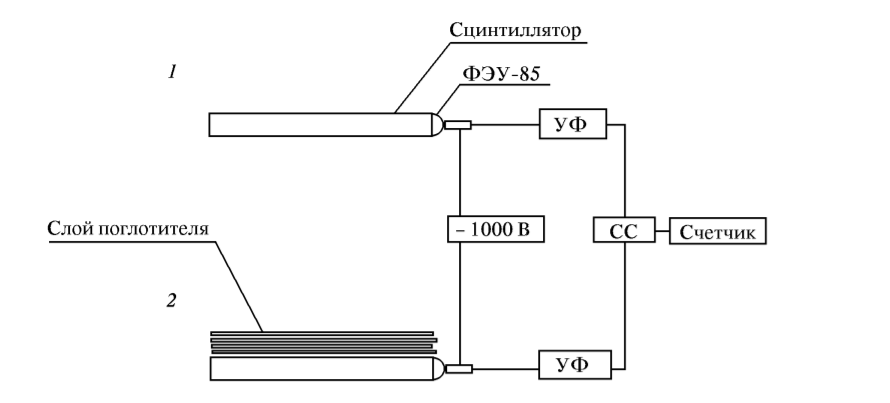
\includegraphics[width=1.0\linewidth]{pics/scheme.png}
    \caption{Схема экспериментальной установки}
    \label{scheme}
\end{figure}    


Регистрация световых вспышек от сцинтилляторов производится с помощью ФЭУ-85,
напряжение питания на каждый ФЭУ подается от стабилизированного высоковольтного
выпрямителя. Сигналы с ФЭУ поступают на усилители-формирователи, а затем на схему
двойных совпадений. Схема совпадений формирует на выходе сигнал только в том
случае, если в обоих детекторах появились сигналы, совпадающие во времени в
интервале, равной разрешающему времени схемы. Число зарегистрированных импульсов
регистрируется пересчетным прибором.


\section{Ход работы и обработка данных}

Ниже представлены результаты измерений, число частиц измерялось за время $t$ = 900 с.

Погрешность измерения штангенциркулем положим $\sigma_{d} = 0,01 \text{ см}$.

Погрешность измерения излучения, будем полагать, находиться в 10\% от измеренной величины. Погрешность обусловлена сложностью процесса излучения. Основное упрощение в нашей модели - учет потери энергии при прохождении через свинцовые пластины.
Поэтому такая большая погрешность. 

\begin{table}[h!]
    \centering
    \begin{tabular}{| c | c | c | c | c |}
\hline
$U, mV$ & $T_{room}, K$ & $T, K$ & $T_{br}, K$ & $ \sigma_{T}, K$\\
\hline
$39920$ & $298$ & $973,66$ & $1000$ & $ 28 $\\
\hline
\end{tabular}

    \caption{: данные для графика}
\label{tb1}
\end{table}

Известно, что мягкая (электронно-фотонная) компонента космического излучения почти
полностью поглощается слоем свинца толщиной 10 - 15 см, а жесткая (мюонная)
практически не поглощается. Имея это в виду, вычитаем из значений $n$ на предыдущем
графике значение, соответствующее $d$ = 131 мм.


\begin{table}[h!]
    \centering
    \begin{tabular}{| c | c | c | c | c |}
\hline
$\theta,^{\circ}$ & $U(I)$ & $V_{ФЭ}$ & $\sigma_{U(I)}$ & $\sigma_{V_{ФЭ}}$\\
\hline
$2404$ & $0,036$ & $0,302$ & $0,0004$ & $0,003$\\
\hline
$$ & $0,032$ & $0,262$ & $0,0004$ & $0,003$\\
\hline
$$ & $0,027$ & $0,202$ & $0,0004$ & $0,003$\\
\hline
$$ & $0,02$ & $0,121$ & $0,0004$ & $0,003$\\
\hline
$$ & $0,016$ & $0,039$ & $0,0004$ & $0,003$\\
\hline
$$ & $0,009$ & $-0,062$ & $0,0004$ & $0,003$\\
\hline
$$ & $0,006$ & $-0,162$ & $0,0004$ & $0,003$\\
\hline
$$ & $0$ & $-0,303$ & $0,0004$ & $0,003$\\
\hline
\end{tabular}

    \caption{: данные для графика}
    \label{tb2}
\end{table}


Построим графики зависимости по таблицам 1, 2.

\begin{figure}[h!]
    \centering
    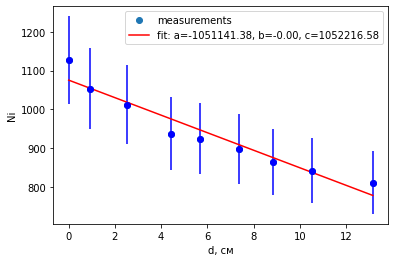
\includegraphics[width=0.8\linewidth]{pics/N_i(d).png}
    \caption{Зависимость числа прошедших частиц от толщины свинца}
    \label{graph}
\end{figure}

\begin{figure}[h!]
    \centering
    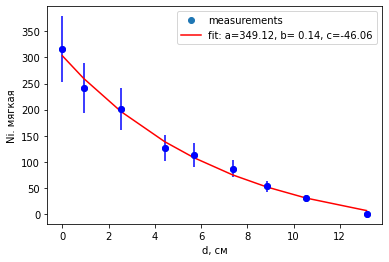
\includegraphics[width=0.8\linewidth]{pics/N_i_light(d).png}
    \caption{Зависимость числа прошедших частиц (мягкая компонента) от толщины свинца}
    \label{graph}
\end{figure}

Заметим, что данные первого графика оказались слишком проблемными для аппроксимации экпонентой, поэтому кривая выродилась в прямую.
В любом случае рассчитаем искомое отношения компонент.

Используя формулу:

\[ \frac{I_м}{I_ж} = \frac{N_{i(d=0)} - N_{i(d=max)}}{N_{i(d=max)}} \]

\[\sigma_{\frac{I_м}{I_ж}} = \frac{I_м}{I_ж} \sqrt{  \left(\frac{\sigma_{N_{i(d=0)}} + \sigma_{N_{i(d=max)}}}{N_{i(d=0)} - N_{i(d=max)}}\right)^{2}  + \left(\frac{\sigma_{N_{i(d=max)}}}{N_{i(d=max)}}\right)^{2}  }  \]

и полученную аппроксимацию с учетом погрешности измерения:

$N_{i(d=0), appox} \approx$ (1075,20 $\pm$ 113) \text{$\frac{част}{см^{2} с}$},  

$N_{i(d=max), appox} \approx$ (777,68 $\pm$ 81) \text{$\frac{част}{см^{2} с}$},  $\Rightarrow$

\[ \frac{I_м}{I_ж} \approx 0,382 \pm 0,046  \]

В пределах погрешности полученное отношение совпадает с теоретических значением, приведенным в теоретическом положении.

\section{Вывод}

В предлжоженной работе была получена зависимость мягкой и жесткой, только мягкой компонент излучения от тольщины свинцовых пластин. В обоих случаях зависимость аппроксимировалась экспонентой. 

График 1 приблизить экспонентой получилось сложнее в виду большего количества частиц $\rightarrow$ большего накопления ошибки.

Из построенной аппроксимации с учетом вычисленных погрешностей получили верхнюю границу отношения мягкой и жесткой компонент.

\textbf{Измереренное значение:}

\[ \frac{I_м}{I_ж} \approx 0,382 \pm 0,046 \]

Полученные результаты хорошо совпадают с теоретическим значением в пределах погрешности.

\textbf{Теоретическое значение:}

\[ {\frac{I_м}{I_ж}}_{theor} \approx 0,412 \]

\end{document}